%!TEX root = ../TFM.tex

\chapter{La Gamificación}


\coment{Esto es lo que correspondería al marco teórico.}


Tras una descripción en términos generales la Gamificación como estrategia metodológica, se tratará de clarificar el concepto de gamificación, porqué y cómo se puede gamificar un contexto para finalizar valorando la aplicación de la gamificación en la educación.


La palabra \textit{Gamificación} es una traducción del término inglés \textit{Gamification}, palabra derivada del sustantivo \textit{game}.
%
En castellano no es posible considerar Gamificación como palabra derivada de otro sustantivo. Por ello, existe otra traducción: ludificación, palabra derivada del adjetivo lúdico.
%
Para el presente trabajo se ha preferido utilizar el término Gamificación para buscar la congruencia con la tendencia de la investigación y el profesorado.


\coment{Qué es la Gamificación}

Según  \cite{GamificationDef}, la \concept[Gamificación]{gamificación} consiste en la utilización de mecánicas, estética y procesos de pensamiento de los juegos para involucrar a las personas, motivar su acción, promover el aprendizaje y resolver problemas.

Esta definición, aunque incluya la promoción del aprendizaje, no está restringida exclusivamente al ámbito educativo. 
%
De hecho, la Gamificación entendida como una estrategia o metodología es aplicada a día de hoy en diversos ámbitos. 
%
Por ejemplo, es una técnica muy utilizada en el campo del Marketing  \citep{GamifyMark} y de los Recursos Humanos  \citep{GamifyHR}.
%
Tanto la Educación, como los Recursos Humanos como el Marketing son contextos no lúdicos en los que es posible utilizar elementos de juegos para involucrar a las personas, motivar su acción, promover el aprendizaje y/o resolver problemas, es decir, para gamificar.

De hecho, la consultora Gartner estudia la Gamificación y tiene su propia definición con algunos matices.
%
Definen gamificación como el uso de mecánicas del juego para impulsar la participación en escenarios no lúdicos, y cambiar comportamientos en un público, con el objetivo de lograr resultados de negocio.
%
Coincide en la utilización de las mecánicas y cambiar comportamientos, sin especificar cuáles, centrándolo todo en lograr resultados de negocio \citep{Gartner}.

Otra definición popular y mucho más general es la que utiliza  \cite{kwerb-WhatIs}: la gamificación es la utilización de elementos de juegos en contextos no-lúdicos.


\coment{Historia de la gamificación}

Gamificación puede ser un término reciente, por ello no hay una única definición consensuada y por ello han sido presentadas diferentes definiciones.
%
Sin embargo, la idea de utilizar las mecánicas de los juegos para resolver problemas y atraer a personas no es precisamente nueva. 
%
En el entorno militar, se llevan utilizando juegos y simulaciones desde hace cientos  de años \citep{GamificationDefII}.

%Otro aspecto novedoso de la gamificación, además del término en sí y su estudio, es su gran crecimiento debido.
%
%Uno de los factores ha sido el auge de la industria del videojuego y la cantidad horas jugadas
%


\coment{Por qué gamificar}

%\paragraph{¿Por qué gamificar?}
Hay bastantes investigaciones recientes que intentan contestar y definir los motivos por los que gamificar o no hacerlo.
%
Recurriendo a una revisión bibliográfica \cite{EmpiricalGamification} se encuentra que la mayoría de experimentos empíricos sobre Gamificación han tenido efectos positivos en términos motivacionales: los participantes han participado más activamente en contextos gamificados que en contextos no gamificados.
%
Sin embargo, no todos los estudios encontraron efectos positivos en todos los participantes.
%
Además, parece que la gamificación falla a largo plazo, tal vez por el efecto de la novedad. 

Pero la gamificación puede producir efectos beneficiosos más allá de la motivación.
% 
De acuerdo con  \cite{kwerb-WhyGamify} la Gamificación permite fidelizar a las personas, hacer todavía más social el contexto, ofrecer a la persona un sentido del progreso en ese contexto y crear un hábito.




%\paragraph{Diferencias entre Juegos serios y Gamificación}

Es importante distinguir gamificación de juegos serios, aunque esta distinción se enfoca de manera distinta según la definición de gamificación elegida.


Los \concept[Juegos serios]{juegos serios} consisten en la modificación del contexto transformándolo en un contexto lúdico \citep{MetaSerious}, mientras que la gamificación incorpora elementos en un contexto no lúdico.
%
Un ejemplo de juego serio sería idear un juego de conquistas como el Risk para trabajar los mapas políticos con los alumnos, mientras que la gamificación consistiría en la implementación de un sistema de recompensas, misiones y otros elementos de los juegos dentro de la clase.

Para \cite{kwerb-WhatIs}, los juegos serios no se deberían considerar como gamificaciones por sus características específicas.
%
Sin embargo, \citep{GamificationDef} sí considera los juegos serios como un subtipo de gamificación.
%
Aunque los juegos serios tengan consecuencias positivas y puedan ser una buena herramienta\footnote{Tanto es así que  \cite{MetaSerious} concluye en su revisión que los juegos serios son más efectivos en contextos de aprendizaje, pero menos efectivo que los métodos convencionales en términos motivacionales.}, su consideración se sale del ámbito del presente trabajo.

\section{Aspectos de la Gamificación}

Un contexto gamificado crea una experiencia y por ello el diseño debe centrarse en la persona.
%
De acuerdo con el ganador del premio \textit{Gamification Guru of the year 2016}\footnote{Premio otorgado en el congreso europeo más grande de Gamificación a nivel internacional, el \gls{WCW}.},  \cite{BeyondPBL}, la gamificación se diseña enfocada en la persona en contraposición con el diseño enfocado en la función o el resultado.
%
La situación se transforma en una experiencia para el usuario, y esta es una de las claves.

Aunque pueda ser una obviedad, en un juego hay jugadores. 
%
No son tratados como participantes ni como usuarios, sino como jugadores.
%
Pensar en las personas participantes de un contexto que se quiere gamificar como jugadores es el primer paso para realizar un diseño enfocado en la persona.
%
Sitúa a esas personas como los protagonistas y como el centro de la experiencia, pues para eso están diseñados los juegos.
%
Además, los jugadores tienen un cierto sentido de autonomía y control sobre la experiencia.

Otra clave a considerar es la siguiente: un juego tiene la meta de que sus jugadores empiecen a jugar, frente a otras posibilidades a su alcance, y se mantengan jugando.
%
Una manera de conseguir esta meta es hacer el recorrido del juego o la experiencia gamificada con una dificultad que se incremente progresivamente y de acuerdo a lo que el jugador puede conseguir en cada momento. 
%
Según el profesor Werbach, es importante que al principio del recorrido sea imposible fracasar, para lo que será necesario diseñar guías y limitar las posibilidades existentes e ir desbloqueándolas a medida que el jugador avanza en la experiencia.


\section{Teorías de base para la Gamificación}

\subsection{Anatomía de la diversión}

Una herramienta muy importante mediante la cual los juegos tienen tanto éxito es la diversión.
%
Es impensable un juego que sea aburrido de jugar.
%
De la misma manera, una gamificación tiene que ser divertida.
%
Es importante esclarecer que hay varios tipos de diversión.
%
De acuerdo con  \cite{whyweplaygames} hay 4 tipos de diversión: 
%
\concept[Diversión\IS Fácil]{Diversión fácil} -- aquella diversión que se produce ante un disfrute de la experiencia, manteniendo la atención del jugador. Se basa en la curiosidad y la intriga --;
%
\label{kindsoffun}
\concept[Diversión\IS Difícil]{Diversión difícil}  -- aquella diversión que producen los retos que requieren habilidad y estrategia más que suerte y que permiten al jugador constatar cuan bueno es--;
%
\concept[Diversión\IS Social]{Diversión social} -- aquella diversión que se fundamenta en la relación con otras personas durante el juego --;
%
\concept[Diversión\IS Interna]{Diversión interna} -- aquella diversión producida por las experiencias internas como el alivio, el entusiasmo y la agitación.

Esta no es la única clasificación de la diversión.
%
En \cite{MDA} se sugiere una división en 8 tipos: sensación, fantasía, narrativa, retos, social, descubrimiento, expresión, pasatiempo.
%
\label{AnatomyOfFun}
%

Esta anatomía de la diversión es fundamental para diseñar una buena gamificación.
%
Un entorno laboral o un contexto educativo normalmente no se caracterizan por ser intrínsecamente divertidos.
%
¿Es posible enfocar la gamificación para trabajar o aprender desde alguna de las dimensiones de la diversión? 


\subsection{Teoría del Flujo} 

La teoría de Csikszentmihalyi investiga e intenta responder a la situación en la que una persona está tan inmersa en una actividad que se olvida de otras circunstancias como el cansancio, el hambre o la incomodidad.
%
A este estado lo llamó \textit{flow}, que en el campo de la Psicología hispanohablante se traduce por \concept[Flujo]{flujo}.
%
\label{autotel}
%
Este estado se produce en actividades autotélicas, es decir, en actividades cuyo fin es la realización de la propia actividad.
%
Las condiciones del flujo incluyen que la percepción de desafío de la tarea y de habilidad sean similares y elevadas, que estén claras las metas intermedias y que se reciba feedback inmediato sobre el progreso \citep{Flow}.
%
En la figura \ref{fig::Flujo} se resumen los posibles estados dependiendo del balance entre el nivel de desafío y la habilidad.

\begin{figure}[hbt]
\begin{center}
\caption{Estados de la teoría del flujo.}
\label{fig::Flujo}
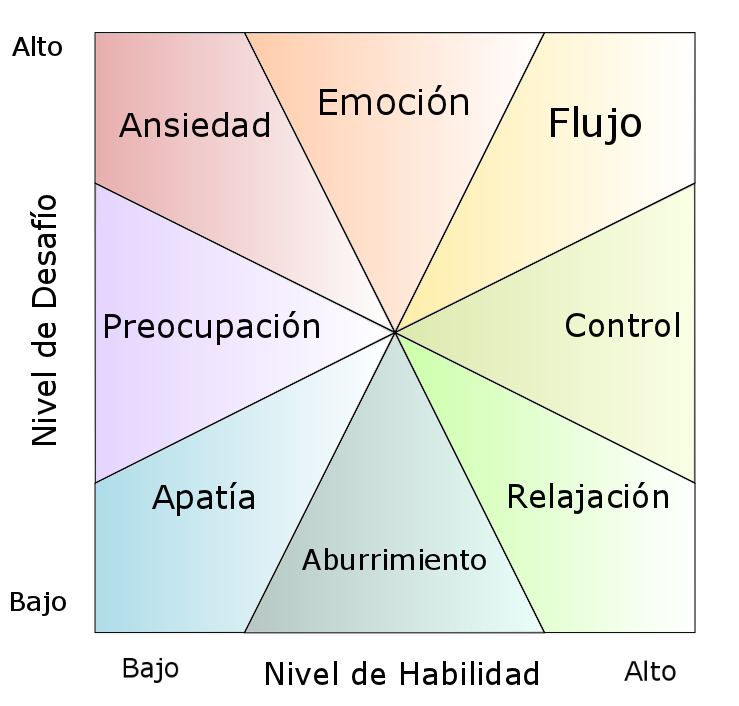
\includegraphics[scale=0.40]{img/Flujo.png}

\small{Fuente: http://www.cluehuntervalencia.com}
\end{center}
\vspace{-0.5cm}
\end{figure}

Csikszentmihalyi entrevistó a jugadores de ajedrez, artistas y deportistas, pero hoy en día, este fenómeno se produce con mucha frecuencia entre los gamers\footnote{Personas con una gran afición por los videojuegos}.
%
La distorsión de la percepción temporal que se produce en el estado de flujo es muy habitual.
%
¿Es posible establecer las condiciones necesarias en un sistema gamificado para que los jugadores entren en estado de flujo?


\subsection{Teoría de la motivación}
\label{SDT}
\label{PosiblesPeligros}
En la Psicología de la Motivación se ha establecido una diferencia entre 2 tipos de motivaciones  \citep{SDT}:  \concept[Motivación\IS Intrínseca]{Motivación intrínseca} -- aquella que depende de los procesos cognitivos internos y está dirigida por el sentido de la autocompetencia, autonomía y relación -- y la \concept[Motivación\IS Extrínseca]{motivación extrínseca} -- aquella que depende de las recompensas que se puedan adquirir con la conducta realizada.
%
Por ejemplo, las actividades autotélicas, mencionadas en la teoría de flujo\crossref{ (ver \ref{autotel})}, necesariamente conllevan una motivación intrínseca.
%
Además de esta diferencia se ha constatado que las conductas motivadas extrínsecamente, sobretodo motivadas con recompensas tangibles, aunque también ocurre con las recompensas verbales, dejan de realizarse cuando desaparece la fuente de motivación, incluso cuando en un momento anterior a la aparición de recompensas la conducta se llevara a cabo motivada intrínsecamente
%
 \citep{ExtrinsicEatsIntrinsic}.

La motivación intrínseca se basa en la \textit{autonomía}, tener la situación bajo control y poder determinar el resultado de las acciones; \textit{competencia} como necesidad de saberse capaz y competente ante los retos y dificultades y \textit{pertenencia} a algo más grande que la propia persona: conectar con otras personas, sentirse parte de la sociedad y compartir los logros.


Es importante conocer esta diferencia a la hora de plantear el objetivo de nuestra gamificación. 
%
Es más sencillo diseñar un sistema de refuerzos basado en el condicionamiento operante, puramente extrínseco que diseñar un sistema que alimente los deseos de autonomía, competencia y pertenencia para fomentar la motivación intrínseca.
%
¿Interesa al diseñador crear un sistema sencillo basado en la motivación extrínseca de los jugadores o, por el contrario, diseñar un sistema más complejo que fomente y haga crecer la motivación intrínseca?



\section{Elementos de la Gamificación}

Tras la exposición de algunas teorías base para la gamificación, se procederá a describir los elementos y las herramientas generales con las que una persona puede diseñar una gamificación para un contexto específico.


\subsection{Pirámide de Werbach}

Los elementos de la Gamificación son los elementos que se encuentran en los juegos, atendiendo a  \cite{werbach2012win} son: dinámicas, mecánicas y componentes, de mayor a menor abstracción.

\concept{Dinámicas} 
%
Las dinámicas son las estructuras implícitas del juego. 
%
Por ejemplo, las reglas serían una manifestación superficial de esa estructura implícita, pero las dinámicas también incluirían manifestaciones conceptuales como podrían ser las restricciones básicas de los juegos, por ejemplo, el respeto a las normas.
%
Se considerarían dinámicas también las emociones, la narrativa, la progresión y las relaciones personales.
%
%\todo{¿Debería incluir alguna definición de los componentes concretos?} 

\concept{Mecánicas} Las mecánicas son los procesos que definen formalmente el contexto y que hacen avanzar la acción. 
%
\label{mecanicas}
%
Por ejemplo, se considerarían mecánicas los retos, la suerte, la competición y la cooperación, el feedback, las recompensas, la adquisición de recursos, las transacciones y los estados de finalización.


\concept{Componentes} Los componentes son las instancias específicas de mecánicas y dinámicas. 
%
Serían componentes los logros, los avatares, los jefes finales\footnote{Batalla muy difícil que tiene lugar al final de cada nivel.}, los combates, el desbloqueo de contenido, los niveles, las misiones, los equipos, las posesiones y el grafo social.
%
Además, hay 3 componentes que merecen una mención específica: los puntos (\textit{points}), las medallas (\textit{badges}) y las clasificaciones (\textit{leaderboards}), comúnmente llamados \gls{PBL}.

Los puntos, por ejemplo, otorgan un feedback acerca del rendimiento y el progreso, es una fuente de datos importante para el diseñador, pueden ligarse con recompensas y se pueden utilizar para determinar los estados de finalización.
%
Las medallas tienen una flexibilidad que permite definir el estilo de un jugador. 
%
Además, tienen un componente social muy importante, ya que muestran el estatus del jugador y son una representación de los logros conseguidos. 
%
También, algunos jugadores se sienten motivados a coleccionarlas.
%
Por último, las clasificaciones o \textit{leaderboards} crean un cierto sentido de competición, en el que los jugadores quieren ascender a puestos más altos de la clasificación, podría ser por el estatus que ofrecen esas posiciones.
%
Se ha estudiado que los \textit{leaderboards} completos desmotivan al 80\% de las personas, debido a la gran brecha que se produce entre los primeros puestos y los últimos.
%
La aproximación más utilizada es diseñar \textit{leaderboards} entre grupos más pequeños de jugadores, por ejemplo, entre los jugadores más cercanos con una puntuación cercana o con sus amigos.



\begin{figure}[hbt]
\begin{center}
\caption{Pirámide de los elementos de Werbach.}
\label{fig::PiramydWerbach}
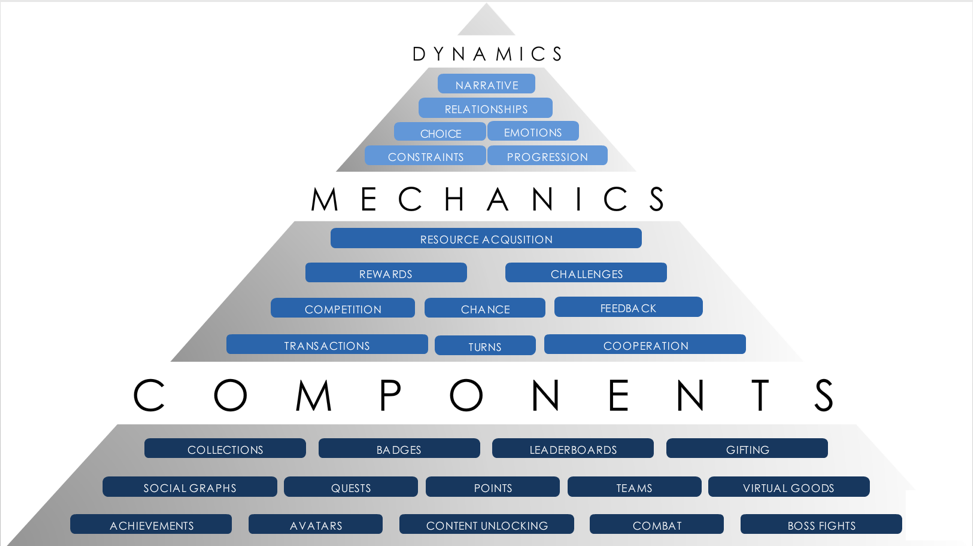
\includegraphics[scale=0.90]{img/Pyramid.png}
\vspace{-0.25cm}
\small{Fuente: \href{http://www.liberty.edu/academics/cafe/index.cfm?id=891255&blogpid=32579&pid=9720}{liberty.edu}.}
\end{center}
\end{figure}
\FloatBarrier



\subsection{Taxonomía de los jugadores}
\label{sec:taxonomy}

\index{Taxonom\'ia de! Bartler}
%
En el proceso de investigación sobre los juegos, sus motivaciones e impactos se ha constatado que no todas las personas responden igual a todos los juegos porque hay tipos de jugadores. 
%
Habiendo distintos tipos de jugadores, no todas las personas responderán por igual a los mismos elementos del juego y habrá elementos más afines a unos tipos de jugadores que a otros. 
%
Por ello, para diseñar correctamente una gamificación es necesario conocer los tipos de jugadores.

Algunas teorías que han tratado de definir una taxonomía de los jugadores, es decir, de clasificar los tipos de jugadores.

 \cite{TypeMUD} estudia a los jugadores de \gls{MUD} según su personalidad y los comportamientos mostrados, según 2 variables: centrados en los jugadores vs centrados el mundo y centrados en la acción y los objetivos del juego vs en la interacción entre jugadores.
%
Estas 2 variables dan lugar a 4 tipos de jugadores, resumido en la imagen \ref{fig::Bartle}:
\begin{itemize}
	\item  \textbf{Triunfadores} (\textit{achievers}): centrados en la acción y en el mundo.
	%
	Tienen un comportamiento individual y quieren llegar a ser los primeros rápidamente.
	

	\item \textbf{Ambiciosos} (\textit{killers}): centrados en la acción y en los jugadores. 
	%
	Estos jugadores buscan las primeras posiciones y además, que los otros jugadores pierdan (de ahí que estén centrados en los jugadores).
	

	\item \textbf{Exploradores} (\textit{explorers}): centrados en la interacción y en el mundo.
	%
	Quieren descubrir y aprender aspectos nuevos del sistema.

	\item \textbf{Sociables} (\textit{socializers}): centrados en la interacción y en los jugadores.
	%
	Juegan para relacionarse con otros jugadores, compartir ideas y experiencias.
\end{itemize}

Se han desarrollado algunos test para clasificar a un jugador en concreto en base a un cuestionario  \cite{Bartletest}.
%
En esta taxonomía no se establece la pertenencia a un tipo único, es decir, una persona puede ser 80\% ambicioso, 15\% triunfador y 5\% explorador.


\begin{figure}[hbt]
\begin{center}
\caption{Taxonomía de los jugadores según Bartle.}
\label{fig::Bartle}
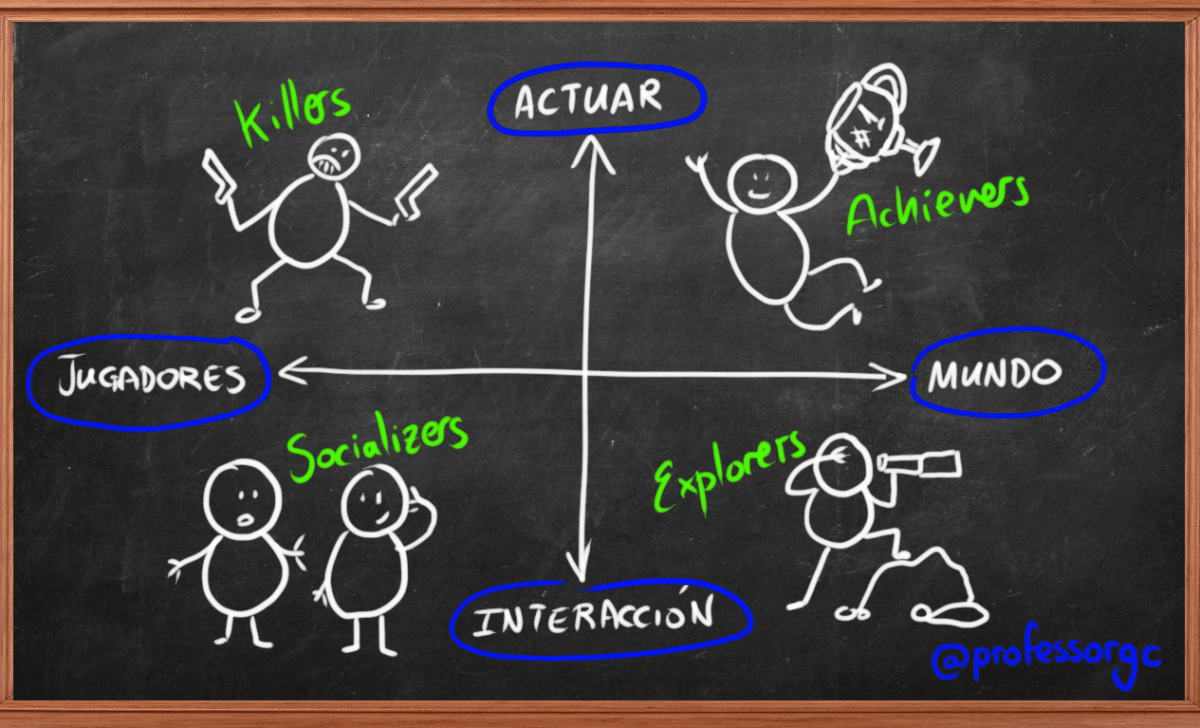
\includegraphics[scale=0.25]{img/Bartle.png}

\vspace{-0.25cm}
\small{Fuente: \url{Creatividadenblanco.com}.}
\end{center}
\end{figure}

Esta clasificación presenta ciertas limitaciones. 
%
La más importante es que se centra en videojuegos \gls{MUD} y, por lo tanto, no es extrapolable a otros juegos; mucho menos a contextos gamificados.
%
Además, el término \textit{killers} en contextos diferentes de videojuegos \gls{MUD} no parece muy adecuado.


\index{Taxonom\'ia de! Amy Jo Kim}
%
Por ello, recurrir a la teoría de  \cite{AmyJoKim}, que se basa en la de Bartle pero la modifica para superar esa limitación.
%
Definen también 4 tipos de jugadores denominados con verbos principales que describen su guía de acción y otros verbos secundarios, como se puede ver en la imagen \ref{fig::AmyJoKim}.
%
La clasificación la hace en base a 2 variables: centrados en el contenido vs centrados en los jugadores y centrados en actuar vs centrados en interactuar.
%
Los jugadores centrados en el contenido y en la actuación serían los competidores (\textbf{compete}), buscando la superación personal.
%
Quienes se centran en el contenido y en la interacción serían los exploradores (\textbf{explore}), buscando el acceso al conocimiento y la información.
%
Los que se centran en los jugadores y en la actuación serían los colaboradores (\textbf{collabore}), buscando formar parte de algo más grande para poder ganar juntos.
%
Por último, las personas que se centran en los jugadores y en la interacción serían los expresivos (\textbf{create}), buscando expresarse, manifestarse y mostrar su creatividad.

\begin{figure}[hbt]
\begin{center}
\caption{Taxonomía de los jugadores según Amy Jo Kim.}
\label{fig::AmyJoKim}
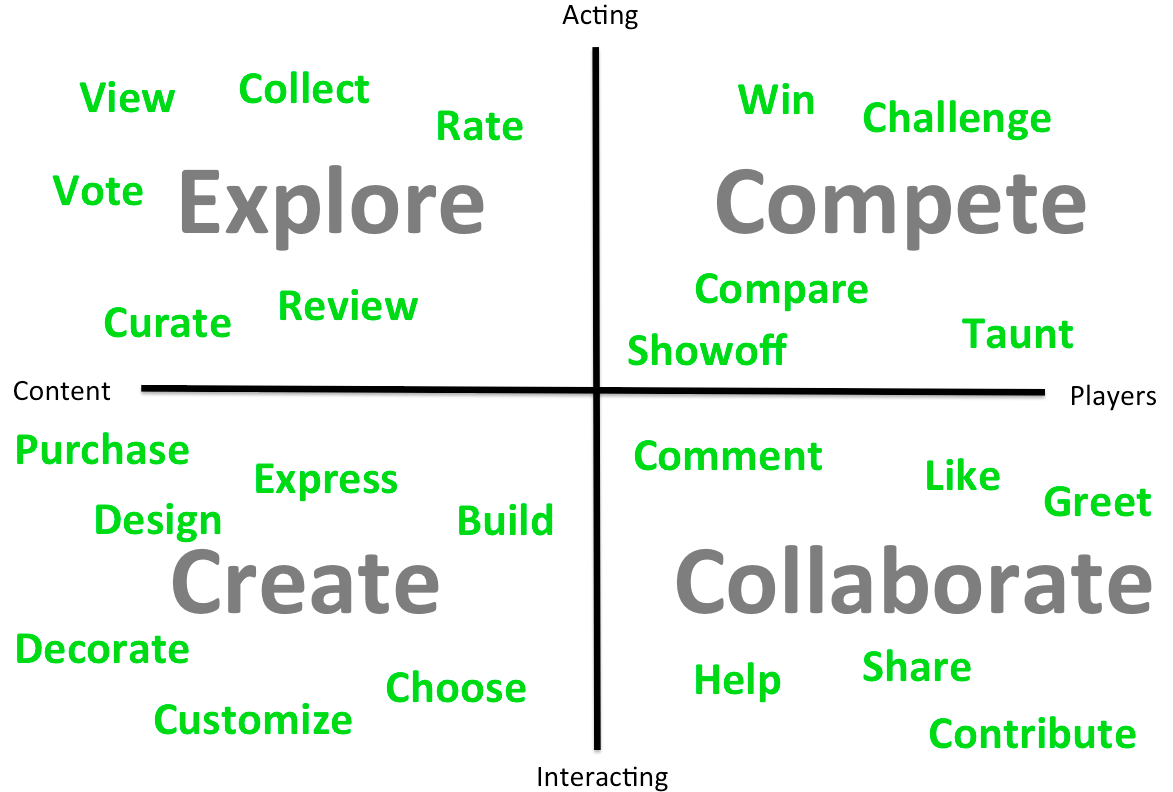
\includegraphics[scale=0.25]{img/AmyJoKim.png}

\vspace{-0.25cm}
\small{Fuente: \url{http://amyjokim.com}.}
\end{center}
\end{figure}


La teoría de Marczewski  \cite{marczewski} es más amplia que las anteriores.
%
Establece más tipos de jugadores, pero además distingue entre jugadores motivados intrínsecamente y extrínsecamente.
%
No sólo eso, sino que los tipos de jugadores motivados extrínsecamente tienen a su vez subgrupos que se parecen a los motivados intrínsecamente, de tal manera que es posible convertir a un jugador motivado extrínsecamente en un jugador motivado intrínsecamente.

En la figura \ref{fig::Marczewski} se puede apreciar el correspondiente esquema de la teoría.
%
En el centro, se encuentra el motivo que guía a cada tipo de jugador. 
%
De estos motivos 4, según  \cite{marczewski} son intrínsecos (Autonomía, Maestría, Relaciones, Propósito\footnote{El único nuevo respecto a la teoría de la auto-determinación  \cite{SDT} es el motivo de \textit{propósito}}) y 2 son extrínsecos: cambio y recompensas.
%
En base a estos 6 motivos, se establecen los 6 tipos de jugadores:
%
Los espíritus libres (\textit{Free spirit}), que son aquellos jugadores que están motivados por la autonomía. Buscan crear y expresarse.
%
Por otro lado, están los triunfadores (\textit{Achiever}), aquellos motivados por la maestría. 
%
Buscan aprender cosas nuevas, mejorar y retos que superar.
%
Quienes están motivados por las relaciones son los socializadores (\textit{Socialiser}).
%
Buscan interactuar con los demás y crear conexiones sociales.
%
El último tipo de jugador motivado intrínsecamente serían los filántropos (\textit{Philantropist}): movidos por el motivo de propósito y significado.
%
Buscan conseguir un propósito que tenga  significado para ellos.
%
Son altruistas y están dispuestos a ayudar a otras personas.
%
Además, se definen los jugadores motivados extrínsecamente, en primer lugar los jugadores (\textit{Player}), motivados por las recompensas. 
%
Harán lo que haga falta para conseguir las recompensas del sistema.
%
A su vez, este tipo de jugador tiene 4 subgrupos: egoísta (\textit{self-esteemer}), consumidor (\textit{consumer}), contacto (\textit{networker}), explotador (\textit{exploitationer}).
%
Para concluir, el último tipo de jugador, también motivado extrínsecamente, sería el perturbador (\textit{Disruptor}) -- aquellos motivados por el cambio. 
%
En general buscan interrumpir el sistema de forma directa o indirectamente (a través de otros usuarios) para forzar el cambio positivo o negativo.
%
Además, este tipo de jugador tiene también 4 subgrupos: influenciador (\textit{influencer}), destructor (\textit{destroyer}), mejorador (\textit{improver}), duelistas (\textit{griefer}).

\begin{figure}[hbtp]
\begin{center}
\index{Taxonom\'ia de! Marczewski}
\caption{Taxonomía de los jugadores según Marczewski.}
\label{fig::Marczewski}
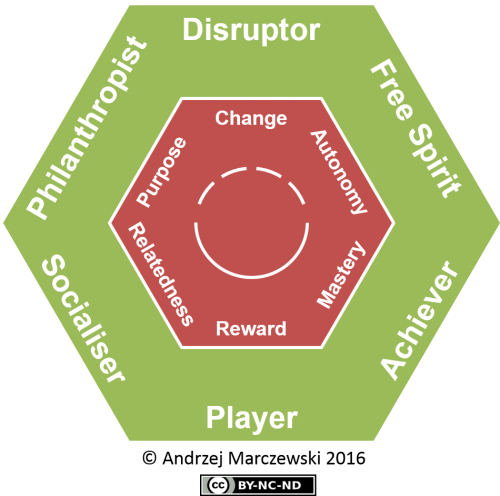
\includegraphics[scale=0.65]{img/Marczewski.jpg}

\vspace{-0.25cm}
\small{Fuente: \url{http://elearningindustry.com}.}
\end{center}
\end{figure}
\FloatBarrier

Como se ha expuesto, esta teoría ofrece un marco de actuación para modificar las motivaciones de los jugadores y transformar a los jugadores extrínsecamente motivados en intrínsecamente motivados.
%
En la figura \ref{fig::MarczewskiEvol} se resume la propuesta de  \cite{marczewski} sobre una posible ruta de evolución de los jugadores para la que, según él, hay cierta evidencia.

\begin{figure}[hbtp]
\begin{center}
\caption{Posible conversión de los jugadores según la taxonomía de Marczewski.}
\label{fig::MarczewskiEvol}
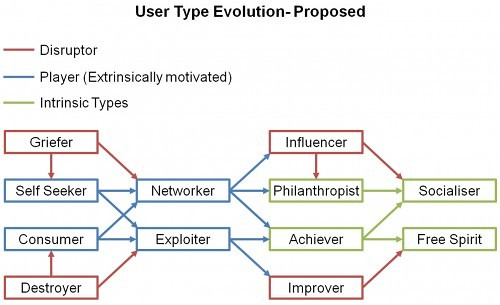
\includegraphics[scale=0.65]{img/evolution.jpg}

\vspace{-0.25cm}
\small{Fuente: \url{http://gamified.uk}.}
\end{center}
\end{figure}
\FloatBarrier





\section{Peligros de la Gamificación}

\subsection{Impacto de la competición en la motivación}


La competición es otra herramienta más a disposición del diseñador, pero es importante tener claro el resultado de algunas investigaciones.
%
Por ejemplo,  \cite{Crawford_CompetitionDef} señala que la competición puede centrar la atención en impedir que el contrincante venza en lugar de centrarse en mejorar y optimizar su propio desempeño.

Otro fenómeno estudiado por  \cite{n-effect} es que el número de competidores y la motivación de los mismos mantienen una relación inversamente proporcional, es decir, cuantos más competidores, menor motivación.

Por último, un estudio llevado a cabo sobre la competición en la educación  \cite{CompetitionInEd} constata que los premios para los ganadores deberían ser de poca importancia o incluso simbólicos para asegurar que el esfuerzo de los estudiantes es intrínseco y no está dirigido por la expectativa del premio.



\subsection{\textit{Pointsification}}

Consiste en la reducción de la gamificación a un simple sistema de puntos en el que se utilizan los aspectos menos esenciales de los juegos y se utilizan como aspectos principales.
%
Los puntos y las medallas en sí no tienen más relación con los juegos que con las páginas web o los programas de fidelización según \cite{Pointsification}.
%
Así, la implementación de una gamificación basada en la mera colección de puntos y medallas no convierte el contexto en divertido ni involucrará a las personas. 
%
Serán necesarios más elementos para llevar a cabo una buena gamificación y no una simple \textit{puntificación}.

\subsection{\textit{Explotationware}}

Un aspecto con el que hay que tener cuidado a la hora de realizar una gamificación es si los futuros jugadores estarían eligiendo libremente participar o no.
%
Si se decidiera utilizar gamificación en una aplicación para fitness, como Nike+, los jugadores que participen lo harán voluntariamente o al menos no obligados por los diseñadores.
%
En cambio, gamificar un entorno laboral o educativo puede resultar más problemático ya que los jugadores pueden perder esa componente de autonomía: no han elegido jugar y por lo tanto su experiencia puede verse perjudicada, fracasando la estrategia.
%
Además, puede no resultar divertido y ser percibido por los trabajadores como una manera de ser controlados y exprimidos en el trabajo.

Un ejemplo de cómo en la gamificación son necesarios muchos más elementos que la competición y las clasificaciones, sería el caso de Disneyland en Anaheim \citep{Explotationware}.
%
En el sótano del hotel, en la lavandería, se colocaron unas pantallas a modo de \textit{leaderboard} con la velocidad de los trabajadores comparados entre ellos.
%
Los trabajadores están listado por el nombre y así, entre compañeros, pueden ver quién es el más rápido haciendo la colada.
%
Lo que podía haberse pensado como una manera de facilitar el trabajo a los operarios, hacerles más agradable el entorno laboral y resolver problemas de eficiencia se había convertido en un desagrado para los trabajadores: éstos se sentían más controlados que antes, ya que sus tiempos estaban continuamente monitorizados y la presión aumentó considerablemente. 
%
Hay trabajadores que cuentan que utilizaban menos el servicio por miedo a aparecer en los últimos puestos de la clasificación.


Con este caso de una gamificación ineficiente, se puede ver que una gamificación mal diseñada no sólo no funciona, sino que es, además, contraproducente. 
%
Una gamificación necesita ser diseñada con cuidado y precisión y eso es lo que va a ser tratado.


